
\chapter{Soluções para Internet of Things}

Nesta secção encontra-se descrita uma pequena introdução ao conceito de \textit{Internet of Things} e respetiva importância no contexto deste projeto. São também apresentadas as principais tecnologias de comunicação possível de utilização e respetiva comparação entre elas. Por fim, serão apresentados alguns projetos/aplicações relacionadas com esta dissertação.  


%a \sr que impulsionará toda esta dissertação. Serão descritas as principais características desta planta, principais propriedades e as diferentes aplicações alimentais existentes no mercado. 



\section{Evolução tecnologia: o IoT}


Antes de descrever a importância e o conceito de \ac{IoT}, é necessário entender as diferenças entre os termos Internet e\ac{WWW}, que 	são usados indistintamente pela sociedade. A Internet é a camada ou rede física composta por \textit{switches}, \textit{routers} e outros equipamentos\cite{Evans2011a}. A sua principal função é transportar informações de um ponto para outro de forma rápida, confiável e segura. Por outro lado, a Web pertence à camada de aplicações que opera sobre a Internet cuja função é oferecer uma interface que transforme as informações que fluem pela Internet em algo útil. Ao longo do tempo, a Web passou e continua a passar por várias etapas evolucionárias, identificadas como:

\begin{itemize}
	\item Web 1.0 – passado: esta primeira etapa foi inventada por Tim Berners Lee em 1989\cite{Getting}. Nesta fase surgiram os principais conceitos que conhecemos da Internet atual: Localizador Uniforme de Recursos (do inglês \ac{URL}), Linguagem de Marcação de Hipertexto (do inglês \ac{HTML}) e Protocolo de Transferência de Hipertexto (do inglês \ac{HTTP}). Ainda nesta primeira fase, mas mais tarde, em 1998 foi criado por Larry Page e Sergey Brin o Google que criou simplicidade nas pesquisas na Web\cite{Lovato2014}. 
	
	\item Web 2.0 – presente: a Web cresceu muito e muito rapidamente. A versão mais próxima da visão de Tim Berners Lee – colaborativa, usado como meio de interação, comunicação global e elevado compartilhamento de informação. 
	
	\item Web 3.0 – futuro: para o futuro prevê-se que os conteúdos online possão vir a estar organizados de forma semântica, muito mais personalizados para cada utilizador, sites, aplicações inteligentes e/ou publicidade baseada nas pesquisas e nos comportamentos.
\end{itemize}

O aparecimento do IoT foi extraordinariamente importante já que se trata da primeira evolução real da Internet, um salto que levará, no futuro, ao desenvolvimento de aplicações revolucionárias com potencial para melhorar significativamente a forma como a sociedade vive, aprende, trabalha e se diverte. O IoT já transformou a Internet em algo sensorial, através da medição de diferentes características, como por exemplo a temperatura, a pressão, as vibrações, a iluminação, a humidade, o stress, entre outras. 

A figura \ref{iotEvolution} representa a evolução da Internet em cinco fases. Inicialmente surge a conexão entre dois computadores que permite a criação de uma rede, posteriormente nasce o conceito de \ac{WWW} ligando um grande número de computadores entre si. Seguidamente, surgiu a Internet móvel que permitiu conectar dispositivos moveis à Internet, possibilitando a ligação da sociedade através das redes sociais.
Finalmente, a internet está a evoluir para o \ac{IoT}, permitindo ligar objetos do quotidiano ao sistema global de redes de computadores \cite{Our2013}.






\begin{figure}[!htb]
	\centering
	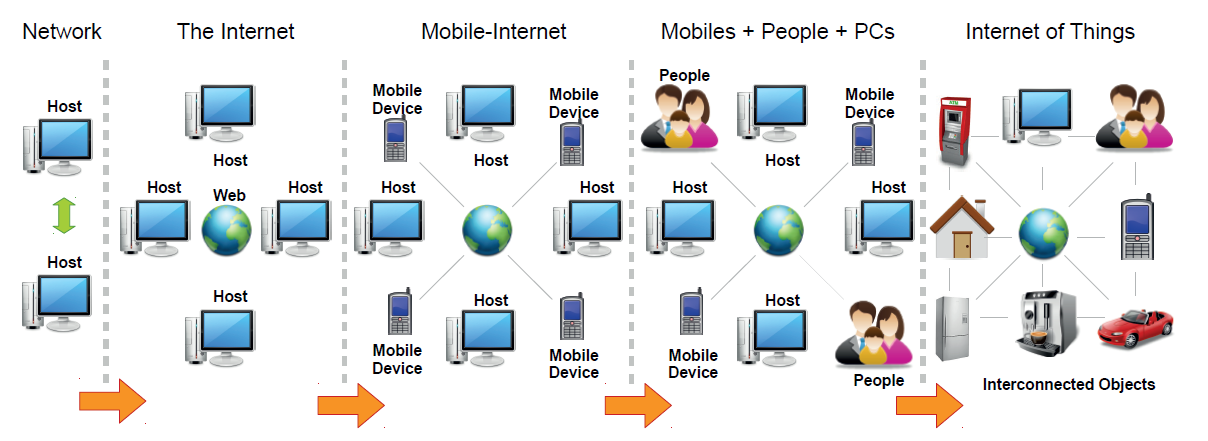
\includegraphics[scale=0.5]{img/cap3-iot/diagrama-evolution.png}
	\caption{Evolução da internet em cinco fases (Adaptado de \cite{Our2013})}
	\label{iotEvolution}
\end{figure}



Uma das principais vantagens do IoT é a sua ligação evidente a todos os objetos, o que por si só é uma ideia avassaladora. O volume de dados gerado por este tipo de ligação pode ser interpretado pelo modelo DIKW que em inglês significa Data-Information-Knowledge-Wisdom \cite{Rowley2007}. Este modelo, também conhecido como pirâmide do conhecimento (Figura \ref{dikw}), é uma hierarquia informacional utilizada especialmente nas áreas da ciência da informação e na gestão do conhecimento, onde cada camada acrescenta certos atributos sobre a anterior.


\begin{figure}[!htb]
	\centering
	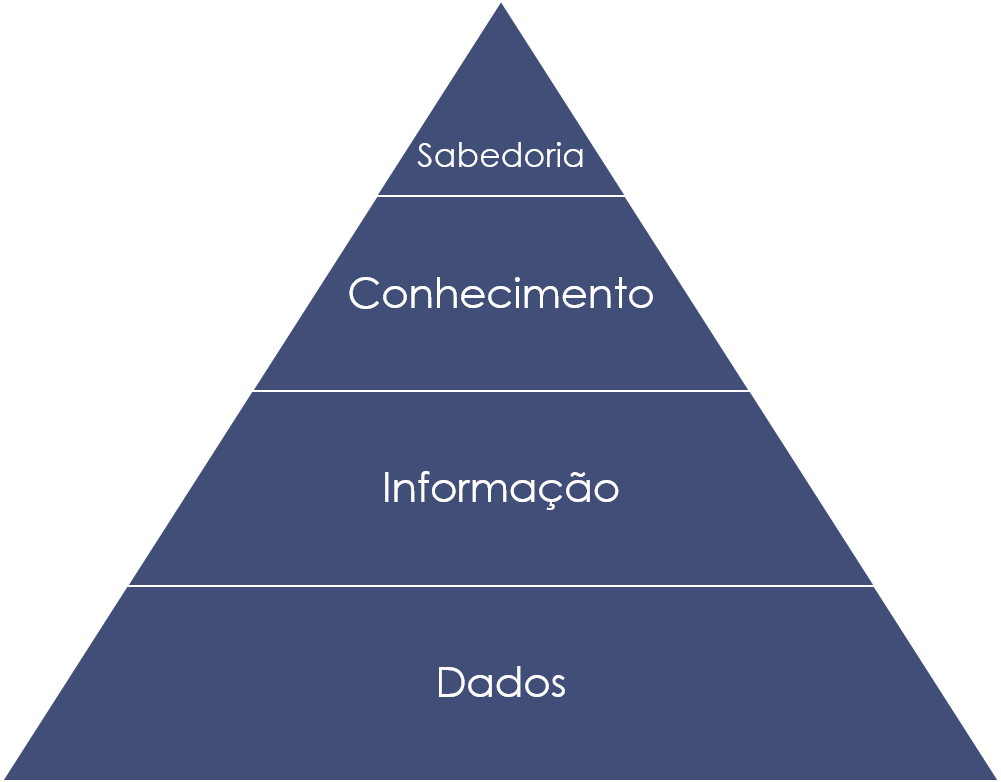
\includegraphics[scale=0.3]{img/cap3-iot/dikw.png}
	\caption{Pirâmide do conhecimento: modelo DIKW}
	\label{dikw}
\end{figure}



A ligação dos objetos à Internet acarreta benefícios visíveis à nossa sociedade, possibilitando um maior controlo e entendimento de como os sistemas interagem entre si e proporcionando uma melhor qualidade de vida a todos. Embora as vantagens se sobreponham às desvantagens não nos podemos esquecer que existem alguns problemas a nível segurança, privacidade, legislação e identidade.


\section{Tecnologias de comunicação usadas em \ac{IoT}}

Nesta secção serão apresentados alguns das tecnologias de comunicação mais utilizados em \textit{Internet of Things} que permite a troca de informações entre dispositivos e respetiva comparação entre eles. 
 

 
\subsection{RFID/NFC}

A identificação por radiofrequência, conhecida por tecnologia \ac{RFID}, é um método de identificação automático através de sinais de rádio. Consiste essencialmente no armazenamento e posterior envio de informação por meio de ondas electromagnéticas para circuitos integrados compatíveis em rádio frequência.  
Os actuais sistemas de \ac{RFID} possuem grande capacidade de identificação e localização de bens ou pessoas levou, o que fez com que esta tecnologia começasse assumisse um papel importante na indústria e no comércio. A comunicação é efetuada entre uma etiqueta, ou marca, e um leitor.


De forma conceptual, o leitor \ac{RFID} é responsável por transmitir um sinal de rádio através da antena para a tag, e esta responde emitindo para o leitor \ac{RFID} o seu \ac{UID}.


\subsection{Bluetooth}

Bluetooth é uma especificação de rede sem fio de âmbito pessoal (Wireless personal area networks – PANs) consideradas do tipo PAN ou mesmo WPAN


\subsection{WiFi}

rede sem fio IEEE 802.11, que também são conhecidas como redes Wi-Fi ou wireless, foram uma das grandes novidades tecnológicas dos últimos anos. Atuando na camada física, o 802.11 define uma série de padrões de transmissão e codificação para comunicações sem fio, sendo os mais comuns: FHSS (Frequency Hopping Spread Spectrun), DSSS (Direct Sequence Spread Spectrum) e OFDM (Orthogonal Frequency Division Multiplexing). Atualmente, é o padrão de fato em conectividade sem fio para redes locais. Como prova desse sucesso pode-se citar o crescente número de Hot Spots e o fato de a maioria dos computadores portáteis novos já saírem de fábrica equipados com interfaces IEEE 802.25. A Rede IEEE possui como principal característica transmitir sinal sem fio através de ondas!


\subsection{Zigbee}

Zigbee designa um conjunto de especificações para a comunicação sem-fio entre dispositivos eletrônicos, com ênfase na baixa potência de operação, na baixa taxa de transmissão de dados e no baixo custo de implementação. Tal conjunto de especificações define camadas do modelo OSI subsequentes àquelas estabelecidas pelo padrão IEEE 802.15.4.


\subsection{LoRa}

A tecnologia Lora

Wide-Area Network Low-Power ( LPWAN ) ou Low-Power Rede ( LPN ) é um tipo de telecomunicações sem fio de rede projetada para permitir comunicações de longo alcance em uma baixa taxa de bits entre as coisas (objetos relacionados), tais como sensores operados em uma bateria.

As tecnologias WAN de baixa potência são projetadas para ambientes de rede máquina a máquina (M2M). Com a diminuição dos requisitos de energia, maior alcance e menor custo do que uma rede móvel, os LPWANs são pensados para permitir uma gama muito mais ampla de aplicativos M2M e Internet of Things (IoT), que foram limitados por orçamentos e problemas de energia.



\subsection{Sigfox}

Uma empresa francesa que constrói redes sem fio para conectar objetos de baixa energia, como medidores de energia elétrica , smartwatches e máquinas de lavar, que precisam estar continuamente ligados e emitindo pequenas quantidades de dados. Sua tecnologia é voltada para a Internet das Coisas (IoT).
 


\subsection{GPRS/GSM}


O \ac{GPRS} é uma tecnologia que aumenta as taxas de transferência de dados nas redes \ac{GSM} existentes. 


Vantagens em relação ao GSM


\subsection{Comparação de tecnologias de comunicação}





\ac{IoT}


\section{Aplicações relacionadas}



Seja para comparar, seja para replicar boas funcionalidades, ou seja para conseguir oferecer algo mais ao utilizador final, quando se pretende desenvolver uma determinada aplicação, e
importante proceder a uma avaliação de aplicações da mesma área se encontram no mercado.
Assim, são aqui abordadas algumas das aplicações relacionadas que são mais utilizadas ou que mais se aproximam daquilo que se pretende para a aplicação a desenvolver neste projeto,
tendo em conta os diferentes sistemas operativos.



\subsection{Multi-monitorização de estufas agrícolas }

https://repositorio.ipcb.pt/bitstream/10400.11/949/1/Multimonitorizacao%20Estufa%20Agricola.PDF

\subsection{Agroopar}

http://www.vidarural.pt/agroopar-os-custos-na-mao-do-agricultor/


\section{Sistema de Monitorização de Estufas Agrícolas}


\cite{Abreu2012}